\documentclass{../paper}

\begin{document}

\title{Identification of Ferromagnets using a Vibrating Sample Magnetometer}

\author{Iago B.~Mendes\,\orcidlink{0009-0007-9845-8448}}
\email{ibrazmen@oberlin.edu}
\affiliation{Department of Physics and Astronomy, Oberlin College, Oberlin, Ohio 44074, USA}

\date{\today}

\begin{abstract}
  In this experiment, we used a Vibrating Sample Magnetometer (VSM) to characterize the magnetic properties of two unknown ferromagnetic samples. By measuring their magnetization curves, we determined their saturation magnetization, which allowed us to identify the materials as Iron and Cobalt. Additionally, we performed a qualitative analysis of the materials in a floppy disk to explore its magnetic behavior. Our results demonstrate the effectiveness of VSM measurements in distinguishing different ferromagnetic materials based on their intrinsic properties.
\end{abstract}

\maketitle

\section{Introduction}

Ferromagnetic materials exhibit unique magnetic behaviors that distinguish them from paramagnetic and diamagnetic materials. One of the defining characteristics of ferromagnets is their ability to retain magnetization even after an external magnetic field is removed. This behavior plays a crucial role in a large set of applications, such as data storage. Understanding these properties requires precise measurement techniques capable of capturing the nature of ferromagnetic responses to external fields.

The Vibrating Sample Magnetometer (VSM) is a widely used instrument for investigating the magnetization characteristics of materials. By vibrating a sample in an applied magnetic field and measuring the induced voltage, the VSM enables the determination of key ferromagnetic features. These measurements can be used in identifying unknown magnetic materials and assessing their suitability for technological applications.

In this experiment, we used a VSM to measure the magnetization curves of two unknown ferromagnetic samples, allowing us to determine their fundamental properties and identify their composition. Additionally, we conducted a qualitative investigation of a floppy disk to observe its magnetic characteristics. In Section \ref{sec:theory}, we provide an overview of magnetization concepts and the different types of magnets. Section \ref{sec:methods} describes the working principles of a VSM and our experimental procedures. Section \ref{sec:results} presents our results and analyses. Finally, we conclude in Section \ref{sec:conclusion} with a summary of our findings and possible areas of improvement.

\section{Theory}\label{sec:theory}

\subsection{Magnetization}

The magnetic properties of a given sample can be described by its magnetic moment $\boldsymbol \mu$, which can be expressed as the maximum torque $\boldsymbol \tau_\text{max}$ on the material when it is in a magnetic flux density $\boldsymbol B$,
\begin{equation}\label{eq:magnetic_moment}
  \boldsymbol \mu = \frac{\boldsymbol \tau_\text{max}}{\boldsymbol B}
\end{equation}
\cite{Jiles}. A possible interpretation of \eqref{eq:magnetic_moment} is that $\boldsymbol \mu$ represents the tendency of aligning with $\boldsymbol B$. To get an intrinsic property of the material, we define the magnetization as the magnetic moment per the sample's volume $V$,
\begin{equation}
  \boldsymbol M = \frac{\boldsymbol \mu}{V},
\end{equation}
or per the sample's mass $m$,
\begin{equation}
  \boldsymbol \sigma = \frac{\boldsymbol \mu}{m}.
\end{equation}

When a sample is put into a magnetic applied field $\boldsymbol H$, it will have a magnetization $\boldsymbol M$ determined by its material properties. Both quantities combine to give the total magnetic flux density $\boldsymbol B$. In SI units, $\boldsymbol B$ is measured in Tesla (T), while $\boldsymbol H$ and $\boldsymbol M$ are measured in amps per meter (A/m), resulting in the relationship
\begin{equation}\label{eq:SI-units}
  \boldsymbol B = \mu_0 (\boldsymbol H + \boldsymbol M)
\end{equation}
\cite{Jiles}, where $\mu_0$ is the permeability of free space.

However, the most common unit system used in the field (and the one used hereafter) is the Gaussian cgs system, in which $\boldsymbol B$ and $\boldsymbol H$ are measured in Gauss (G), while $\boldsymbol M$ is measured in electromagnetic units per cubic centimeter (emu/cm$^3$) \cite{QuantumDesign}. In these units, \eqref{eq:SI-units} becomes
\begin{equation}\label{eq:cgs-units}
  B = H + 4\pi M
\end{equation}
\cite{QuantumDesign}. Note that the bold symbols were dropped in \eqref{eq:cgs-units} to indicate that we will be concerned only with the magnitudes of these quantities along a given direction.

\subsection{Magnet Types}

We can categorize different types of magnets based on how their magnetization $M$ responds to changes in the applied field $H$. Figure \ref{fig:MH-curves} shows the behavior of four distinct magnets.

We identify a {\em paramagnet} by a linear, reversible $M(H)$ curve with positive-slope for which $M(0) = 0$ \cite{QuantumDesign}. Similarly, a {\em diamagnet} also has a linear, reversible $M(H)$ curve with $M(0) = 0$, but it has a negative slope \cite{QuantumDesign}. Since $M$ can be interpreted as the tendency to align with $H$, this means that paramagnets tend to align with $H$ whereas diamagnets tend to anti-align with $H$.

In striking contrast, a {\em ferromagnet} is described by a non-linear, non-reversible $M(H)$ curve \cite{QuantumDesign}. Magnetic hysteresis is a common term used to describe this lack of reversibility \cite{QuantumDesign}. As indicated by Figures \ref{fig:soft-ferromagnet} and \ref{fig:hard-ferromagnet}, such hysteresis implies that $M(0) \neq 0$ if the curve is followed from large values of $H$. In other words, after removing the applied field $H$, a ferromagnet retains a remanent magnetization. To reduce the magnetization to zero, an opposite field must be applied until $M(H_c) = 0$. The value of $H_c$ to make this happen is called coercivity. Ferromagnets with small coercivity (as in Figure \ref{fig:soft-ferromagnet}) are called soft, while ferromagnets with large coercivity (as in Figure \ref{fig:hard-ferromagnet}) are called hard.

Another key feature of ferromagnets is that the $M(H)$ curve asymptotes to a saturation magnetization $M_s$. This is an intrinsic property of magnetic materials, which we exploit to identify our samples.

\begin{figure}
  \centering
  \begin{subfigure}{0.45\columnwidth}
    \centering
    \begin{sketch}[
      xlabel = {$H$},
      ylabel = {$M$},
    ]
      \addplot[very thick, domain = 0:10] {x};
    \end{sketch}
    \caption{Paramagnet}
    \label{fig:paramagnet}
  \end{subfigure}
  \begin{subfigure}{0.45\columnwidth}
    \centering
    \begin{sketch}[
      xlabel = {$H$},
      ylabel = {$M$},
    ]
      \addplot[very thick, domain = 0:10] {-x};
    \end{sketch}
    \caption{Diamagnet}
    \label{fig:diamagnet}
  \end{subfigure}
  \begin{subfigure}{0.45\columnwidth}
    \centering
    \begin{sketch}[
      xlabel = {$H$},
      ylabel = {$M$},
      samples = 100
    ]
      \addplot[very thick, domain = -10:10] {tanh((x-0.5))};
      \addplot[very thick, domain = -10:10] {tanh((x+0.5))};
    \end{sketch}
    \caption{Soft ferromagnet}
    \label{fig:soft-ferromagnet}
  \end{subfigure}
  \begin{subfigure}{0.45\columnwidth}
    \centering
    \begin{sketch}[
      xlabel = {$H$},
      ylabel = {$M$},
      samples = 100
    ]
      \addplot[very thick, domain = -10:10] {tanh((x-4))};
      \addplot[very thick, domain = -10:10] {tanh((x+4))};
    \end{sketch}
    \caption{Hard ferromagnet}
    \label{fig:hard-ferromagnet}
  \end{subfigure}

  \caption{Qualitative sketches of the expected magnetization $M$ versus applied field $H$ for different magnet types.}
  \label{fig:MH-curves}
\end{figure}

\section{Methods}\label{sec:methods}

To quantitatively measure curves like the ones in Figure \ref{fig:MH-curves}, we use a VSM. Figure \ref{fig:VSM} shows a picture of the VSM used in this experiment with indications to the main components.

\begin{figure}
  \centering
  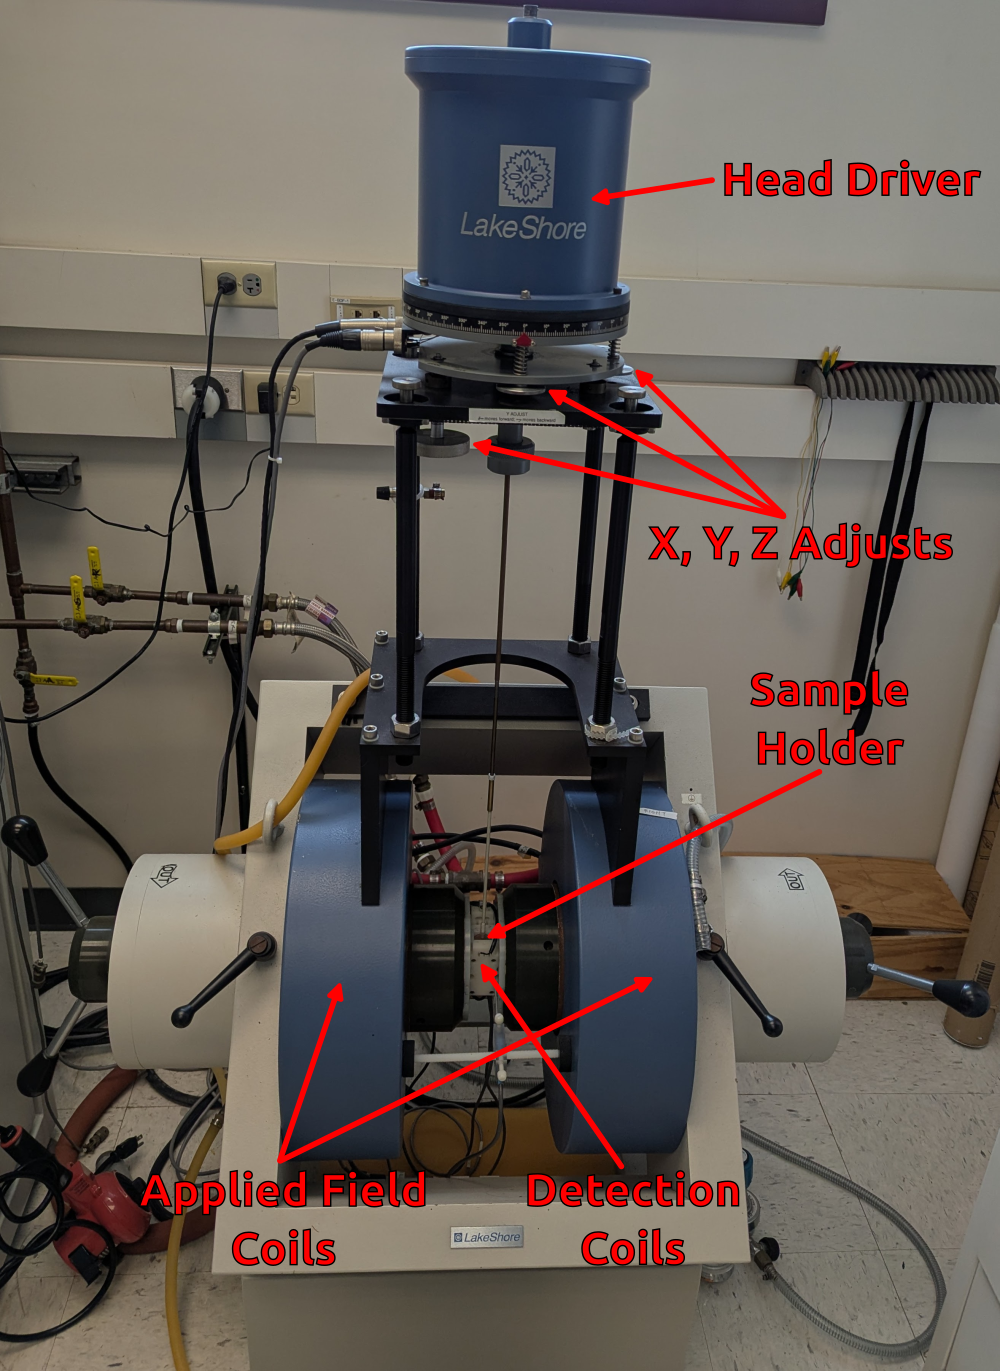
\includegraphics[width=0.9\columnwidth]{data/VSM.png}
  \caption{Picture of the VSM with indications to the main components.}
  \label{fig:VSM}
\end{figure}

The VSM exploits Faraday's Law of Induction, where a changing magnetic flux induces a voltage in an electrical circuit \cite{Jiles}. By mechanically vibrating the sample perpendicular to an applied field, the VSM generates an alternating magnetic flux, which is detected and converted into the sample's magnetic moment. The vibration is set by the head driver, which is connected to the sample holder by a rod. The applied field $H$ is created by running current through a set of coils that surround the sample. Another set of coils is used to detect the induced current from the vibrating sample.

After inserting a sample into the VSM, we need to carefully center it using the x, y, and z adjusts. This is a critical step because the output of the detection coils depends on the position of the sample \cite{Oxford}. We use a ``saddling'' technique, in which we look for a maximal signal in z, a minimum signal in x, and a maximum signal in y (in this order) \cite{LabManual}. The x-axis here is taken to be the line going through the center of the applied field coils. Hence, finding the minimum signal in x is equivalent to placing the sample at equal distance from these coils. Additionally, the reason why we maximize the signal in y and z is because we want to place the sample in the line connecting these coils and any deviations from it cause a weaker magnetization. To get a sense of how much uncertainty is involved in this process, we centered the VSM twice for each sample, collecting data after each centering.

To calibrate the VSM, we used a Nickel (Ni) standard with known magnetic moment. This gave us a conversion factor between the measured voltage in the detection coils and the sample magnetic moment equal to $801$ emu/mV. Looking at previous Ni calibrations done on the same VSM by other groups, we see a variation of this conversion factor on the order of $\sim 5\%$, which introduces a significant error in our experiment.

\section{Results}\label{sec:results}

We refer to the first unknown sample we measured as element A. The results from the first run are shown in figure \ref{fig:elementA}. This first run had a saturation value of $\mu^{A1}_{s+} = 8.4405$ emu for positive $H$ and $\mu^{A1}_{s-} = -8.3559$ emu for negative $H$. In the second run, we had a saturation value of $\mu^{A2}_{s+} = 8.5734$ emu for positive $H$ and $\mu^{A2}_{s-} = -8.4498$ emu for negative $H$. In theory, we expect $\mu^{Ai}_{s+} = |\mu^{Ai}_{s-}|$ for $i \in \{1,2\}$. That is, the saturation absolute values should be the same for both positive and negative $H$. The difference between these values in our data indicates an imperfect centering when setting up the VSM. Taking the average of these four values and using the $\sim 5\%$ uncertainty from calibration, we find a saturation magnetic moment of
\begin{equation}
  \mu_s^A = 8.5(4) \text{ emu}.
\end{equation}
Additionally, we measured the mass of element A to be
\begin{equation}
  m^A = 0.0403(1) \text{ g}.
\end{equation}
Therefore, we have a saturation mass magnetization of
\begin{equation}\label{eq:elementA}
  \sigma_s^A = \frac{\mu_s^A}{m^A} = 210(10) \text{ emu/g}.
\end{equation}
The value in \eqref{eq:elementA} is closest to the literature value for Iron (Fe), which has a saturation mass magnetization of 218.0 emu/g at $20\deg$C \cite{CRCHandbook}.

We refer to the second unkonwn sample we measured as element B. The results from its first run are shown in figure \ref{fig:elementB}. Note that it is clear from this curve that the sample did not reach saturation for an applied field of 10,000 G, which is near the limit of our VSM. To address this, we can fit the data points using the Langevin function -- an expression from the classical theory of paramagnetism that serves as an approximation to the ferromagnet curves \cite{LabManual} --, which can be written as
\begin{equation}
  L(x) = \coth(x) - \frac{1}{x}
\end{equation}
\cite{CullityGraham}. To do this, we use {\tt SciPy}'s {\tt optimize.curve\_fit} procedure \cite{SciPy}, which finds the coefficients $A$ and $B$ that make function $A L(B x)$ the best fit for the given data points. The resulting fits are shown in figure \ref{fig:fits}. Since
\begin{equation}
  \lim_{x \to \infty} L(x) = 1,
\end{equation}
the coefficient $A$ gives us the saturation magnetic moment of each fit. In figure \ref{fig:fit1}, we have $A=5.70$. In figure \ref{fig:fit2}, we have $A=5.67$. Taking the average of these values and using the $\sim 5\%$ uncertainty from calibration, we find element B's saturation magnetic moment to be
\begin{equation}
  \mu_s^B = 5.7(3) \text{ emu}.
\end{equation}
Additionally, we measured element B's mass to be
\begin{equation}
  m^B = 0.0321(2) \text{ g}.
\end{equation}
Therefore, we have
\begin{equation}\label{eq:elementB}
  \sigma_s^B = \frac{\mu_s^B}{m^B} = 180(10) \text{ emu/g}.
\end{equation}
The value in \eqref{eq:elementB} is closest to the literature value for Cobalt (Co), which has a saturation mass magnetization of 161 emu/g at $20\deg$C \cite{CRCHandbook}. Note that $\sigma_s^B$ is near the edge of two standard deviations from the literature value, which indicates that the extrapolation done using the Langevin function is not a good model.

Finally, our third sample was a piece of a floppy disk, for which we aim to make only a qualitative analysis. The results are shown in figure \ref{fig:floppy}. From this curve, we see that the floppy disk is made out of a ferromagnet with an intermediate coercivity, which is especially important for a storage device. That's because the data bits in a floppy disk are physically stored as remanent magnetizations pointing either ``up'' or ``down''. If it was a very soft ferromagnet, each bit would easily change its orientation, losing its information. If it was a very hard ferromagnet, it would require a very strong applied field in order to flip the magnetization of the bits when writing information. By being in-between these extremes, the floppy disk can effectively be used to store data.

\begin{figure*}
  \centering
  \begin{subfigure}{\columnwidth}
    \centering
    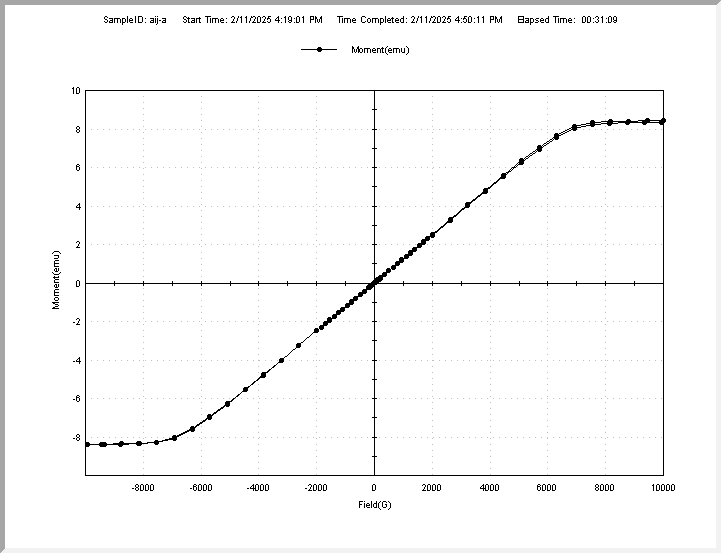
\includegraphics[width=\textwidth]{data/aij-a-2-11-0.png}
    \caption{Element A}
    \label{fig:elementA}
  \end{subfigure}
  \begin{subfigure}{\columnwidth}
    \centering
    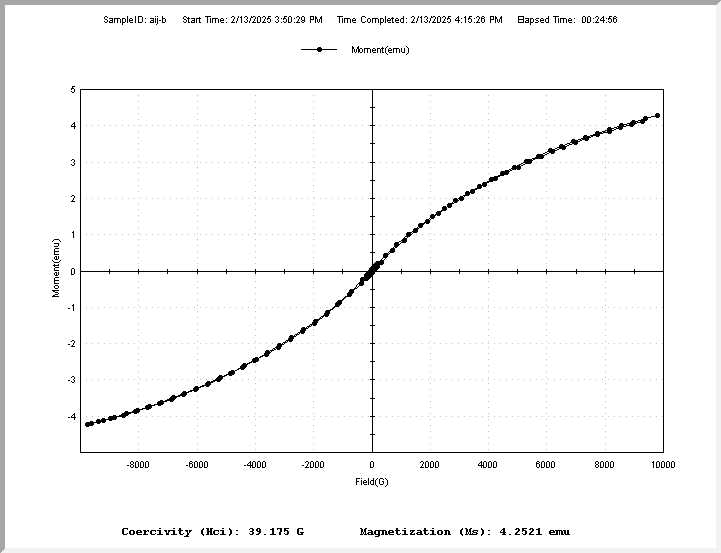
\includegraphics[width=\textwidth]{data/aij-b-2-13-0.png}
    \caption{Element B}
    \label{fig:elementB}
  \end{subfigure}

  \begin{subfigure}{\columnwidth}
    \centering
    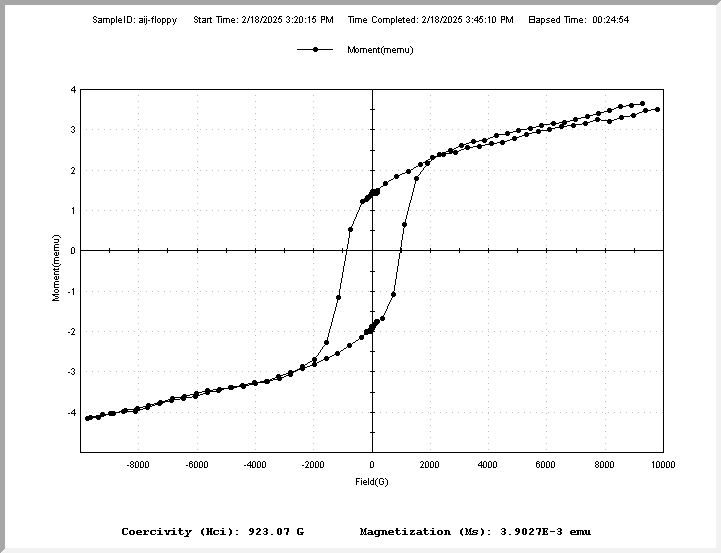
\includegraphics[width=\textwidth]{data/aij-floppy-2-18-0.png}
    \caption{Floppy disk}
    \label{fig:floppy}
  \end{subfigure}

  \caption{Magnetic moment $\mu$ versus applied field $H$ for the two unknown ferromagnets and for a piece of a floppy disk.}
  \label{fig:AB-curves}
\end{figure*}

\begin{figure*}
  \centering
  \begin{subfigure}{\columnwidth}
    \centering
    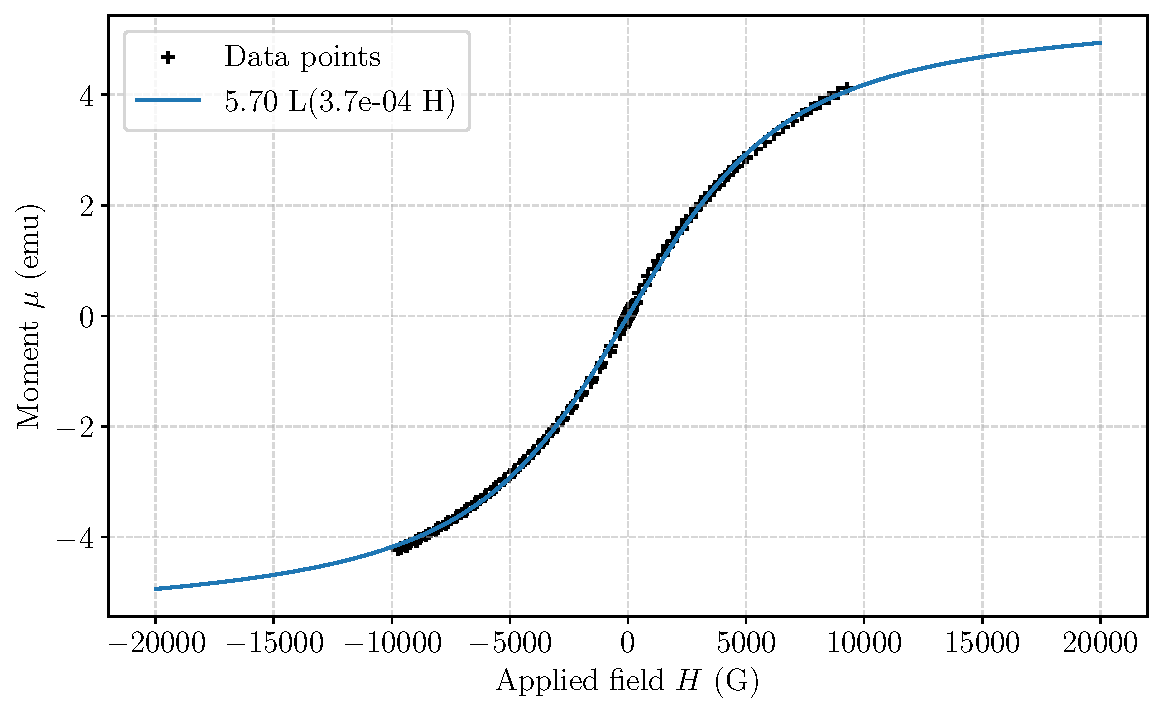
\includegraphics[width=\textwidth]{data/aij-b-2-13-0-data-fit.pdf}
    \caption{First run}
    \label{fig:fit1}
  \end{subfigure}
  \begin{subfigure}{\columnwidth}
    \centering
    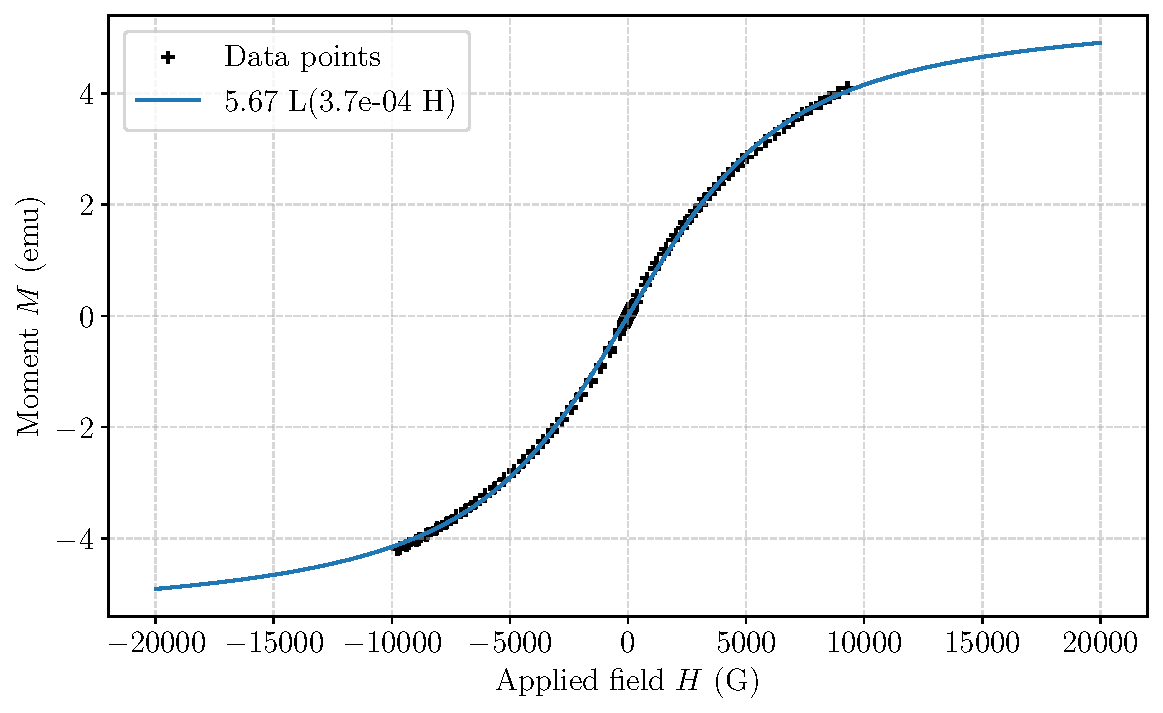
\includegraphics[width=\textwidth]{data/aij-b-2-13-1-data-fit.pdf}
    \caption{Second run}
    \label{fig:fit2}
  \end{subfigure}

  \caption{Fit of element B's curve using the Langevin function $L(x)$.}
  \label{fig:fits}
\end{figure*}

\section{Conclusion}\label{sec:conclusion}

Using a Vibrating Sample Magnetometer (VSM), we successfully characterized the magnetic properties of two unknown ferromagnetic materials and identified them as Iron and Cobalt based on their saturation magnetization. The measured hysteresis curves provided insight into the intrinsic properties of the samples, demonstrating the utility of VSM techniques in material identification. Furthermore, our examination of a floppy disk highlighted the role of magnetism in data storage. These results reinforce the importance of precise magnetic measurements.

It is worth noting that we have only used the  error from calibration for the uncertainties of the VSM output. The reason for this is that such error is much more significant than any of the other variations in our data. In future experiments, it would be useful to perform multiple calibrations instead of depending on a single one, as this could improve the accuracy and reliability of the measurements. Additionally, further investigation into other sources of error, such as sample positioning and temperature fluctuations, could refine the precision of VSM measurements.

\begin{acknowledgements}
  This work was done in collaboration with Avay Subedi and John Duffy under the supervision of Professor Yuri Ijiri.
\end{acknowledgements}

\bibliography{refs}

\end{document}
